\documentclass[%
reprint,
%superscriptaddress,
%groupedaddress,
%unsortedaddress,
%runinaddress,
%frontmatterverbose,
%preprint,
%showpacs,preprintnumbers,
%nofootinbib,
%nobibnotes,
%bibnotes,
amsmath,
amssymb,
aps,
pra,
%prb,
%rmp,
%prstab,
%prstper,
%floatfix,
showkeys
]{revtex4-1}

\renewcommand{\figurename}{Figure}
\renewcommand{\tablename}{Table}

\usepackage[utf8]{inputenc}
\usepackage{colortbl}
\usepackage{graphicx}
\usepackage{hyperref}
\usepackage{ulem}

\usepackage{epstopdf}


\usepackage{feynmp}
\DeclareGraphicsRule{*}{mps}{*}{}

% \makeatletter
% \def\endfmffile{%
% \fmfcmd{\p@rcent\space the end.^^J%
%         end.^^J%
%         endinput;}%
% \if@fmfio
%    \immediate\closeout\@outfmf
% \fi
% \ifnum\pdfshellescape=\@ne
%    \immediate\write18{mpost \thefmffile}%
% \fi}
% \makeatother

\begin{document}


% Use the \preprint command to place your local institutional report
% number in the upper righthand corner of the title page in preprint mode.
% Multiple \preprint commands are allowed.
% Use the 'preprintnumbers' class option to override journal defaults
% to display numbers if necessary
%\preprint{}

%Title of paper
\title{Activities Report for the 3rd year of the FCT PhD Fellowship SFRH/BD/77979/2011}

% repeat the \author .. \affiliation  etc. as needed
% \email, \thanks, \homepage, \altaffiliation all apply to the current
% author. Explanatory text should go in the []'s, actual e-mail
% address or url should go in the {}'s for \email and \homepage.
% Please use the appropriate macro foreach each type of information

% \affiliation command applies to all authors since the last
% \affiliation command. The \affiliation command should follow the
% other information
% \affiliation can be followed by \email, \homepage, \thanks as well.
\author{João Pela}
\email[]{joao.pela@cern.ch}
%\homepage[]{Your web page}
%\thanks{}
%\altaffiliation{}
\affiliation{Imperial College London}

%Collaboration name if desired (requires use of superscriptaddress
%option in \documentclass). \noaffiliation is required (may also be
%used with the \author command).
%\collaboration can be followed by \email, \homepage, \thanks as well.
%\collaboration{}
%\noaffiliation

\date{\today}

\begin{abstract}
Theoretical and experimental motivations are presented for the analysis
in which I am involved at the Compact Muon Solenoid experiment, the standard model Higgs on the $\gamma\gamma$ decay 
channel analysis and vector boson fusion produced Higgs with invisible decay products analysis. A summary of the 
service work already performed is also given.
\end{abstract}

% insert suggested PACS numbers in braces on next line
%\pacs{}
% insert suggested keywords - APS authors don't need to do this
\keywords{Experimental high energy physics, trigger systems and data acquisition}

%\maketitle must follow title, authors, abstract, \pacs, and \keywords
\maketitle

\setlength{\unitlength}{1mm}

\section{Physics introduction}

The current knowledge on the field of particle physics is summarized in the standard model (SM). It is known that
this model is incomplete without the inclusion of a spontaneous symmetry breaking mechanism that would explain
the observation that the electroweak bosons (the W and Z particles) have mass. The easiest way to introduce such
a mechanism is with the Higgs mechanism, which suggests the presence of a new particle, the Higgs boson.

After 3 years of successful operation, the experiments built on the Large Hadron Collider (LHC) at European Organization 
for Nuclear Research (CERN) located near Geneva, Switzerland observed of a new boson. Measurements of properties of this 
new particle are compatible within uncertainties with what would be expected for a SM Higgs boson.

The Compact Muon Solenoid experiment (CMS) published results where the best-fit signal strength for a SM Higgs boson 
mass hypothesis of 125 $GeV$ is $\sigma_{SM}=0.87\pm0.23$. The excess is most significantly seen in the $\gamma\gamma$ 
and in the ZZ decay channel, which together are the channels with best mass resolution. A fit to these signals gives 
a mass of $125.3 \pm 0.4 (stat.) \pm 0.5 (syst.)$ $GeV$. The decay to two photons indicates that the new particle is 
a boson with spin different from 1\cite{article:CMS-HIG-12-028}.

The ATLAS collaboration also presented simultaneously similar results and claim of a new neutral boson
with a measured mass of $126.0 \pm 0.4 (stat.) \pm 0.4 (syst.)$ $GeV$ \cite{article:CERN-PH-EP-2012-218}.

\subsection{Higgs phenomenology}

The main processes for Standard Model Higgs production are summarized in figure \ref{table_HiggsDiagrams}.
 
\begin{figure}[floatfix]
 
\begin{tabular}{cc}
\begin{fmffile}{feynmanDiagram_GFHiggs}
\fmfframe(0,5)(0,5){
\begin{fmfgraph*}(30,20)
   \fmfleft{g1,g2} \fmfright{H'}
   \fmf{gluon}{g1,t1}
   \fmf{gluon}{g2,t2}
   \fmf{fermion,tension=0,label=$t$,label.side=left}{t1,t2}
   \fmf{fermion,label=$t$,label.side=left}{t2,H}
   \fmf{fermion,label=$\bar{t}$}{H,t1}
   \fmf{boson}{H,H'}
   \fmflabel{$H^0$}{H'}
   \fmflabel{$g_1$}{g1}
   \fmflabel{$g_2$}{g2}
\end{fmfgraph*}
}
\end{fmffile}

(1) &

\begin{fmffile}{feynmanDiagram_VBFHiggs}
\fmfframe(0,5)(0,5){
\begin{fmfgraph*}(30,20)
   \fmfleft{P1,P2} \fmfright{P1',H',P2'}
   \fmf{fermion}{P1,g1}
   \fmf{fermion}{P2,g2}
   \fmf{boson,label=$W/Z^0$,label.side=left}{g1,H}
   \fmf{boson,label=$W/Z^0$,label.side=left}{H,g2}
   \fmfdot{H,g1,g1}
   \fmf{boson,tension=0.2}{H,H'}
   \fmf{fermion}{g1,P1'}
   \fmf{fermion}{g2,P2'}
   \fmflabel{$H^0$}{H'}
   \fmflabel{$q_1$}{P1}
   \fmflabel{$q_2$}{P2}
   \fmflabel{$q_1'$}{P1'}
   \fmflabel{$q_2'$}{P2'}
\end{fmfgraph*}
}
\end{fmffile}
(2) \\
\begin{fmffile}{feynmanDiagram_ttFHiggs}
\fmfframe(0,5)(0,5){
\begin{fmfgraph*}(30,20)
   \fmfleft{g2,g1}
   \fmfright{t2',H',t1'}
   \fmf{gluon}{g2,t2}
   \fmf{gluon}{g1,t1}
   \fmf{fermion}{t2',t2}
   \fmf{fermion,label.side=right,label=$t$}{t2,H}
   \fmf{fermion,label.side=right,label=$\bar{t}$}{H,t1}
   \fmf{fermion}{t1,t1'}
   \fmf{boson,tension=0.5}{H,H'}
   \fmflabel{$H^0$}{H'}
   \fmflabel{$g_1$}{g1}
   \fmflabel{$g_2$}{g2}
   \fmflabel{$t$}{t1'}
   \fmflabel{$\bar{t}$}{t2'}
\end{fmfgraph*}
}
\end{fmffile}
(3) &

\begin{fmffile}{feynmanDiagram_WZstrahlung}
\fmfframe(0,5)(0,5){
\begin{fmfgraph*}(30,20)
   \fmfleft{q2,q1} \fmfright{H',V'}
   \fmf{fermion}{v1,q2}
   \fmf{fermion}{q1,v1}
   \fmf{boson,label=$W/Z$}{v1,v2}
   \fmf{boson}{v2,V'}
   \fmf{boson}{v2,H'}
   \fmflabel{$H^0$}{H'}
   \fmflabel{$W/Z$}{V'}
   \fmflabel{$q$}{q1}
   \fmflabel{$\bar{q}$}{q2}
\end{fmfgraph*}
}
\end{fmffile}
(4)

\end{tabular}

\label{table_HiggsDiagrams}
\caption{Main processes for standard model Higgs production ordered by highest cross section at the LHC. (1) gluon 
fusion,(2) vector boson fusion, (3) $t\bar{t}$ fusion and (4) $W/Z$ associated production.}
\end{figure}

The respective cross sections for each production process can be found in figure \ref{figure_SMHiggs_XSec}
\cite{Takahashi:1019873}. It can be seen that the gluon fusion (GF) is the leading process by almost one order of
magnitude higher than vector boson fusion (VBF) which is the second most frequent process in the currently allowed 
experimental mass range for a Standard Model Higgs Boson. Both $t\bar{t}$ fusion and weak boson associated productions 
have cross sections more than one order of magnitude lower than VBF in the same mass range.

\begin{figure}[ht]
\centering
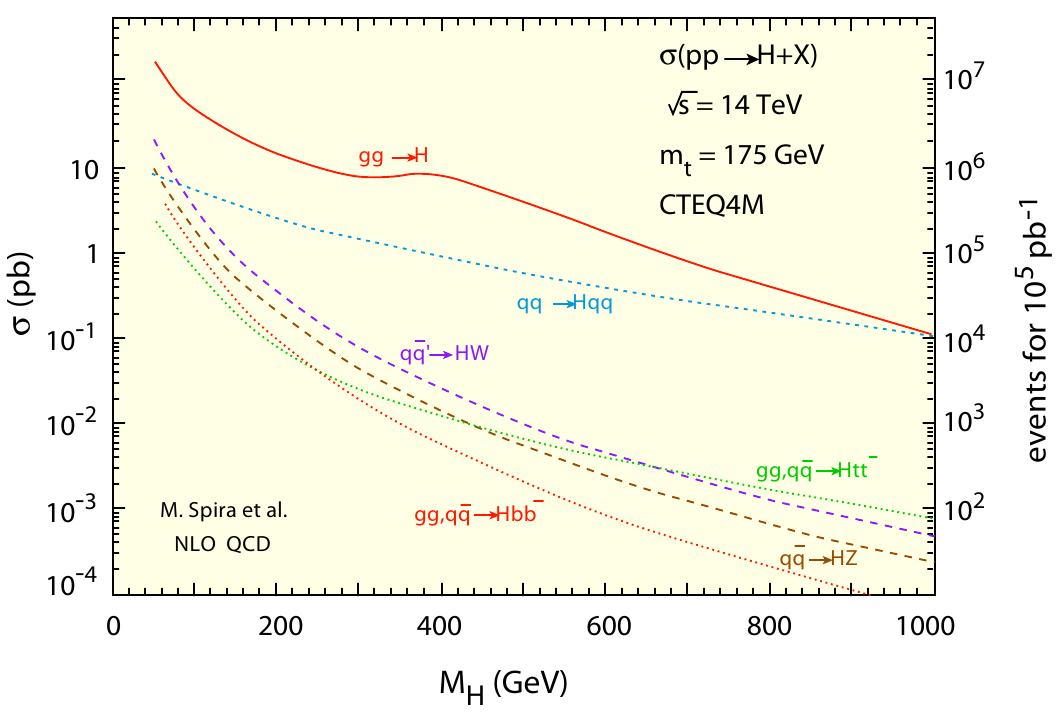
\includegraphics[width=0.45\textwidth]{img/SMHiggs_XSec.png}
\caption{Theoretical prediction of standard model Higgs productions cross sections for a $\sqrt(s)=14$ $TeV$
and assuming $m_{top}=175$ $GeV$.}
\label{figure_SMHiggs_XSec}
\end{figure}

The Higgs boson will then decay with different probabilities to different objects depending on its mass; a plot
of these probabilities can be found at figure \ref{figure_SMHiggs_BR} \cite{Takahashi:1019873}.

\begin{figure}[ht]
\centering
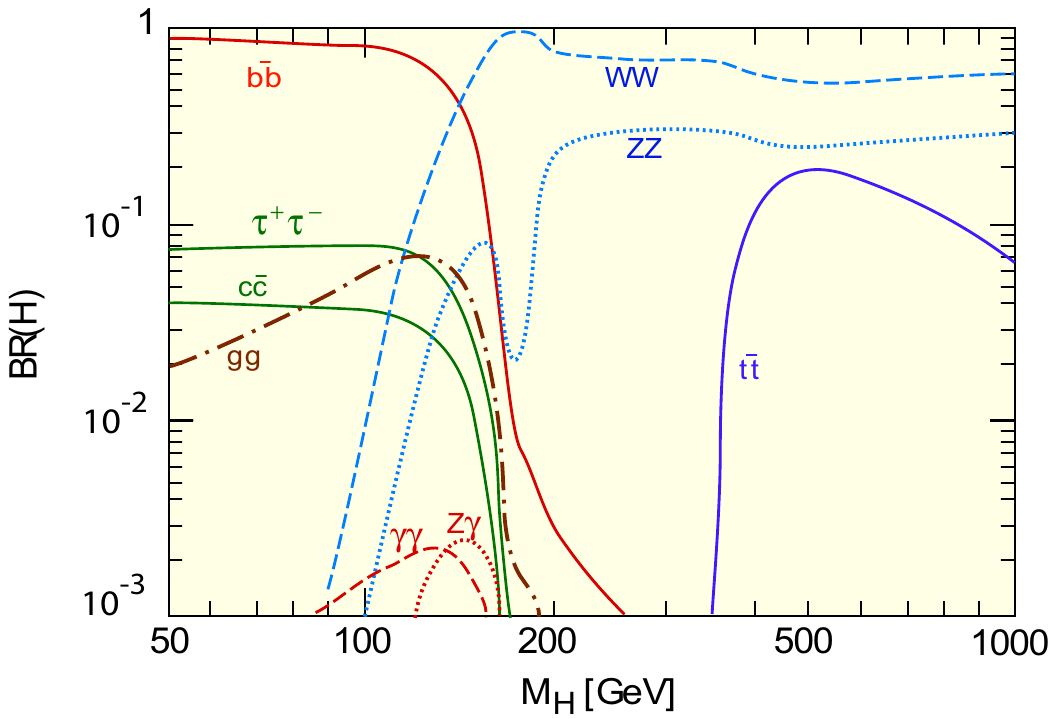
\includegraphics[width=0.45\textwidth]{img/SMHiggs_BR.png}
\caption{Theoretical prediction of standard model Higgs branching ratios as a function of its mass.}
\label{figure_SMHiggs_BR}
\end{figure}

\subsection{Higgs to \texorpdfstring{$\gamma\gamma$}{gamma-gamma}}

The $H \rightarrow \gamma\gamma$ channel main production mechanism is gluon fusion. This process compared with the 
other possible production mechanisms and decays is the one that presents the biggest potential for discovery at low
masses, since its clean signature and amount of background on the signal area make this channel the most promising.

In the $H \rightarrow \gamma\gamma$ analysis a search is made for a narrow peak in the diphoton invariant mass
distribution in the range 110–150 GeV. This signal is sitting on a large irreducible background from QCD production 
of two photons and reducible background where one or more of the reconstructed photons originate from 
misidentification of jet fragments.

\subsection{Vector boson fusion Higgs to invisible}

The first theoretical motivations for looking for VBF Higgs events is obviously to observe and measure its
cross section and each of the branching ratios for its decays. We can then calculate its coupling to the
weak bosons and to fermions (including the leptonic sector via $\tau\bar{\tau}$). From the couplings, we may be able 
to differentiate between a SM Higgs or beyond the standard model (BSM) Higgs such as one of the super symmetric
incarnations of this boson\cite{article:Duhrssen:2004cv,article:Zeppenfeld:2000td}. Also for models where the Higgs 
would only decay invisibly, VBF is the primary discovery channel.

From the experimental point of view, we can see from figure \ref{figure_SMHiggs_XSec} that VBF has a cross section
one order of magnitude lower than GF, but we should notice from diagram 2 in figure \ref{table_HiggsDiagrams} that
there are two forward jets produced along with the Higgs and we can use them for tagging. 

Also, we can profit from the lack of colour exchange between the interacting quarks which will result in low 
hadronic activity in the central rapidity region coming from the main interaction. Since the Higgs visible decay 
products (if any) are most likely produced in the central rapidity region, this means that they will be likely 
isolated from the forward jets thus allowing better reconstruction/identification efficiency which should allow 
easier study of the Higgs properties.

In the case of an invisible decay we can profit from the large Z to invisible decay branching ratio. On the other hand
we do not have the Higgs decay products to reconstruct its mass, so we have to rely only on the missing energy and 
tagged jets to identify these events.

\section{Experimental introduction}

\subsection{Large Hadron Collider}

The Large Hadron Collider (LHC) is at this moment the world's largest and highest-energy particle accelerator
in activity. It was built in a 27 kilometer circular tunnel, at an average depth of around 100 meters, under the
Franco-Swiss border near Geneva, Switzerland\cite{Bruning:2004ej}.

The LHC is a synchrotron machine designed to accelerate and collide two opposing particle beams.
Particles are injected into the machine in bunches, which can be composed of protons or lead nuclei. For
protons the maximum nominal energy that can be achieved per beam is 7 $TeV$, which represents 14 $TeV$ in the
center of mass frame for a single proton-proton collision. For lead nuclei a maximum nominal energy of
574 $TeV$ per nucleus (2.76 $TeV$ per nucleon) per beam is planned. The running conditions for proton collisions
during 2012 are 8 $TeV$ center of mass energy, with an initial average number pile up collisions
of the order of 28 and a delivering instant luminosity of the order of $5 \times 10^{33}$ $cm^{-2}s^{-2}$

\subsection{Compact Muon Solenoid}

The Compact Muon Solenoid experiment (CMS) is a general purpose experiment that is an integrating part of the LHC
program. It was designed to study the collisions of two intersecting proton beams in its centre 
\cite{article:CMSTDRv12006}. This detector was planned with the intention of studying a broad spectrum of physics 
processes and is made of several subsystems, each one designed to take advantage of some characteristics of the 
particles produced in order to measure their energy, momentum and charge. The detector has classical onion structure 
with several layers. Starting from the collision point outwards we have: pixel system, tracker system, electromagnetic 
calorimeter, hadronic calorimeter, magnet, muon systems and return yoke.

At nominal conditions, forty million collisions are produced in a single second and it would be impossible to
register all of them. As almost all collisions are uninteresting, the solution is to have an event selection
already in the machine so we would only save the most interesting events. This is the role of the trigger system,
which is split into two levels, where the second level benefits from the extra time from the selection at first 
level to access more information of what happened. Using this approach by stages we are able to reduce the number 
of events to a more manageable rate between of under 1500 $Hz$.

The overall dimensions of CMS detector are a length of 21.6 $m$, a diameter of 14,6 $m$, and total weight of
12500 $tons$.

\subsection{Trigger}

\subsubsection{Run I (2012-13)}

During run I (2012-13) the LHC was run with $50$ $ns$ bunch separations leading to a maximum bunch crossing rate of approximately 20 $MHz$. 
Data from only about $10^3$ $events/sec$ can be written to archival media; hence, the trigger system has to achieve a
rejection factor of $\sim 2 \times 10^5$ by selecting what may be the most interesting events. The CMS trigger and data 
acquisition system consists of: the detector electronics, the Level-1 trigger processors (calorimeter, muon, and global), 
the readout network, and an online event filter system (processor farm) that executes the software for the High-Level 
Trigger (HLT).

\subsubsection{Run II (2015-)}

Following two year of technical stop for repair and upgrade the LHC will resume operations. The accelerator itself
will be increasing its energy from 4 $TeV$ per beam to 6.5 $TeV$ and will be able to run with bunch separations
of only 25 $ns$, potentially doubling the number of collisions per second. The CMS experiment also underwent an upgrade
program to make use of this new conditions offered by the LHC. 

\subsection{Level 1 trigger}

The size of the LHC detectors and the underground caverns imposes a minimum transit time for signals from
the front-end electronics to reach the services cavern housing the Level-1 trigger logic and return back to the
detector front-end electronics. The total time allocated for the transit and for reaching a decision to keep or
discard data from a particular beam crossing is 3.2 $\mu s$. During this time, the detector data must be held in
buffers while trigger data is collected from the front-end electronics and decisions are reached. This decision
allows to discard a large fraction of events while retaining the small fraction of interactions of interest (nearly
1 crossing in 1000) at hardware level. Of the total latency, the time allocated to Level-1 trigger calculations
is less than 1 $\mu s$.

\section{Data Analysis}

\subsection{Vector Boson Higgs to Invisible}

\subsubsection{VBF Signature at CMS}

The VBF SM Higgs signature main characteristic is the presence of two forward jets associated with the Higgs 
(see diagram 2 in figure \ref{table_HiggsDiagrams}). These two forward jets have a reasonable $p_T$ ($\gtrsim30$ $GeV$), 
high $\Delta\eta$ separation between them ($\gtrsim 3)$ and low $\Delta\phi$ ($\lesssim 2.5$).
The dijet pair also has a high invariant mass since it will be produced back-to-back to the Higgs boson. Because there
is no color exchange between the incoming quarks, the hadronic activity between the jets is suppressed. On the other
hand, the Higgs decay products, if any, will be located at the central rapidity area which will be easier to 
study because of the lower hadronic activity coming from the main interaction already 
described\cite{article:Dokshitzer:1991he}. 

To illustrate this separation of the SM Higgs decay products let's look at VBF Higgs decay to a pair of $\tau$.
The distribution of the pseudo-rapidity for both forward jets and two $\tau$ coming from SM Higgs decay of simulated 
events at the CMS detector can be found in figure \ref{figure_VBF_HToTauTau_ObjectsRapidityGap}.

\begin{figure}[ht]
\centering
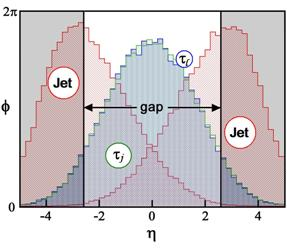
\includegraphics[width=0.45\textwidth]{img/ObjectsRapidityGap.jpeg}
\caption{Simultaneous plot of the $\eta$ coordinate of both forward jets and the $\tau\bar{\tau}$
produced from simulated VBF Higgs decay. Super-imposed with 4 circles showing the possible positions of these 4
objects in a hypothetical event.}
\label{figure_VBF_HToTauTau_ObjectsRapidityGap}
\end{figure}

The CMS detector is ideal for these types of searches since it is a $4\pi$ hermetic detector with calorimeter coverage
from -5 to 5 in pseudo-rapidity. It also has very good capabilities of particle measurement and identification which 
can be used to identify the forward jets and Higgs decay products or in case of an invisible decay, compute the 
resulting missing transverse energy. An event display of a simulated Standard Model Higgs (which then decays to 
$\tau\bar{\tau}$) produced via VBF can be found in figure \ref{figure_EventDisplay_VBF_HToTauTau_El-Had}.

\begin{figure}[ht]
\centering
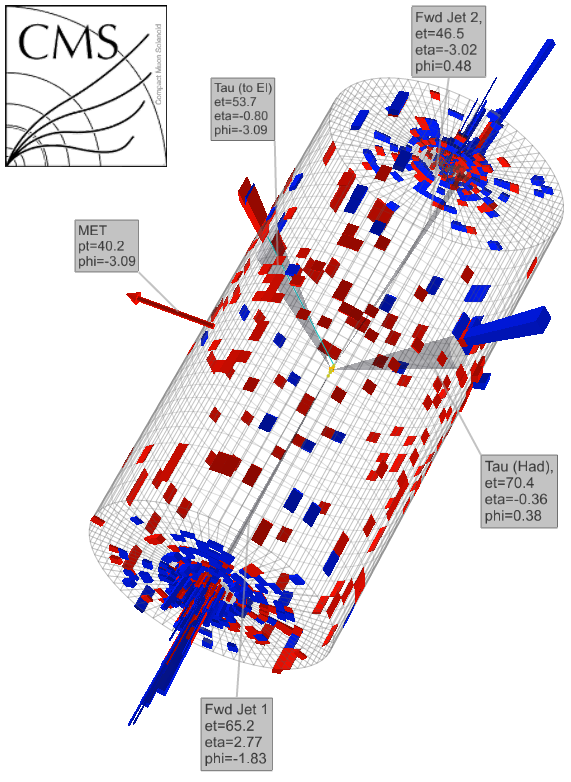
\includegraphics[width=0.45\textwidth]{img/EventDisplay_VBF_HToTauTau_El-Had.png}
\caption{Event display of a simulated event where a standard model Higgs is produced via vector boson fusion
which then decays to $\tau\bar{\tau}$, this in turn decay leptonically to an electron (left) and hadronically (right).}
\label{figure_EventDisplay_VBF_HToTauTau_El-Had}
\end{figure}


\subsubsection{Invisible Higgs trigger}


\subsection{Study of variables for QCD suppression}

One of the most difficult background to estimate in the VBF Higgs to invisible analysis is QCD. This is mostly due to
the lack of Monte Carlo sample statistics which are very difficult to produce because of the enormous quantity of events 
necessary to replicate enough signal like QCD.

A possible approach is to try to reduce QCD levels where it can be considered negligible. In an attempt to use this 
approach we started to look for possible new variables that with a minimal signal impact would reduce QCD event yields
by several orders of magnitude. 

Three new variables were studied which try to exploit the correlations of the dijet plus MET system: Scalar Tri-Object 
Sum, Dijet pT fraction and Vector Tri-Object Sum.  
  
\subsubsection{Scalar Tri-Object Sum}

This variable is defined as $|pT(jet1)|+|pT(jet2)|+|MET|$ which is similar to HT but only applied to our objects of
interest. This implies that the higher it is, the better the average relative object resolution. This variable can also
be used to relax constraints on individual object while still enforcing a global minimum transverse energy of the 
combined system.

\subsubsection{Dijet \texorpdfstring{$p_{T}$}{pT} fraction}

This variable is defined as $p_{T}(dijet)/(p_{T}(dijet)+MET)$. It reflects the balance of the dijet plus MET system.
For signal it should peak strongly around 0.5 while this should not be the case for QCD in the case MET is faked.

\subsubsection{Vector Tri-Object Sum}

This variable is defined as $|Vector Sum(pT(jet1)+pT(jet2)+MET)|$. It also reflects the balance of the dijet plus MET
system. In this case, value of the variable for signal should concentrate around zero with the spread defined by the
jet and MET resolution. The possibility of using jet and MET resolution as an input to this variable is being studied. 
 
\subsubsection{Combining variable}

Based on the method of some CMS SUSY analysis that use an HT cut in conjunction with the $\alpha_T$ variables, a 
study was performed to evaluate the possibility of combining the scalar tri-object sum with each of dijet plus MET 
variables. Two dimensional plots for the signal monte carlo after the MET cut on the official VBF to invisible
analysis can be seen in fig \ref{figure_MET_dijetFrac_htMET_VBFInv} for dijet $p_T$ fraction versus scalar tri-Object 
sum and fig \ref{figure_MET_vecSum_htMET_VBFInv} for vector tri-object sum versus scalar tri-object sum.


\begin{figure}[ht]
\centering
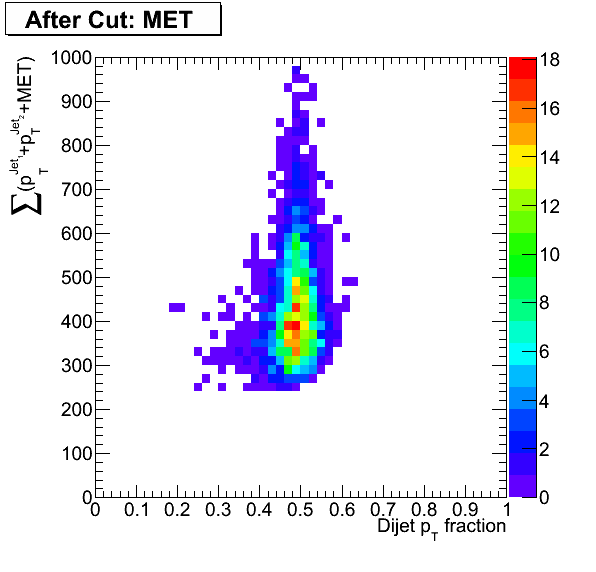
\includegraphics[width=0.45\textwidth]{img/MET_dijetFrac_htMET_VBFInv.png}
\caption{Plot of dijet $p_T$ fraction versus scalar tri-object sum for signal monte carlos $m_H=120$ $GeV$ after the
         MET cut of the official VBF to invisible analysis.}
\label{figure_MET_dijetFrac_htMET_VBFInv}
\end{figure}

\begin{figure}[ht]
\centering
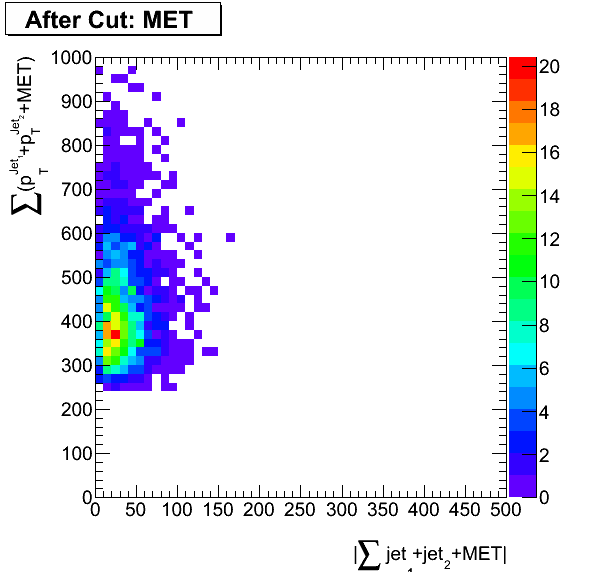
\includegraphics[width=0.45\textwidth]{img/MET_vecSum_htMET_VBFInv.png}
\caption{Plot of vector tri-object sum versus scalar tri-object sum for signal monte carlos $m_H=120$ $GeV$ after the
         MET cut of the official VBF to invisible analysis.}
\label{figure_MET_vecSum_htMET_VBFInv}
\end{figure}

Preliminary studies show that by defining a 2D cut on these pairs of variables could yield a reduction of a factor of
2.5 on QCD, Z+Jet and W+Jets with a signal loss of less than 30\%. 

These studies may prove especially valuable for use in parked data, since by applying constraints on this type of system
variables we may be able to relax cut on jet $p_T$ and MET and therefore increase signal yield making use of the lower 
trigger thresholds for these individual objects, while keeping or even improving signal to background ratio.

\section{Run II Preparation}


\begin{widetext}
\centering
\vspace{2cm}
\rule{8cm}{.1pt} \\
Joao Pela (Student)

\vspace{2cm}
\rule{8cm}{.1pt} \\
David Colling (Supervisor)

\end{widetext}

\bibliographystyle{abbrv}
\bibliography{Renewal_4th_Year_Bibliography}




\end{document}
